\documentclass{beamer}

% Theme and color
\usetheme{Madrid}
\usecolortheme{seahorse}

% Packages
\usepackage{graphicx}
\usepackage{amsmath}
\usepackage{hyperref}
\usepackage{listings}
\usepackage{xcolor}
\usepackage{tikz}
\usepackage{booktabs}

% Define colors
\definecolor{codegreen}{rgb}{0,0.6,0}
\definecolor{codegray}{rgb}{0.5,0.5,0.5}
\definecolor{codepurple}{rgb}{0.58,0,0.82}
\definecolor{backcolour}{rgb}{0.95,0.95,0.92}

% Code listing settings
\lstset{
    basicstyle=\tiny\ttfamily,
    keywordstyle=\color{blue},
    commentstyle=\color{codegreen},
    stringstyle=\color{codepurple},
    showstringspaces=false,
    breaklines=true,
    frame=single,
    backgroundcolor=\color{backcolour},
    numbers=left,
    numberstyle=\tiny\color{codegray}
}

% Title page information
\title{$\varepsilon$-Differential Privacy Query Estimation with LLMs}
\subtitle{Privacy-Preserving Database Statistics Generation}
\author{Seth Lupo}
\institute{Tufts Security and Privacy Lab\\
\texttt{seth.lupo@tufts.edu}}
\date{July 28, 2025}

% Remove navigation symbols
\setbeamertemplate{navigation symbols}{}

\begin{document}

% Title slide
\begin{frame}
\titlepage
\end{frame}

% Outline slide
\begin{frame}{Outline}
\tableofcontents
\end{frame}

% Section 1: Introduction and Motivation
\section{Introduction and Motivation}

\begin{frame}{Database Query Optimization}
\frametitle{The Role of Statistics in Query Planning}

\begin{block}{Query Optimization Pipeline}
\begin{enumerate}
    \item Parse SQL query into abstract syntax tree
    \item \textbf{Use table statistics to estimate costs}
    \item Generate multiple query execution plans
    \item Select plan with lowest estimated cost
    \item Execute the selected plan
\end{enumerate}
\end{block}

\vspace{0.5cm}

\begin{alertblock}{Why Statistics Matter}
\begin{itemize}
    \item Determine optimal join order in multi-table queries
    \item Choose between sequential scan vs. index scan
    \item Estimate memory requirements for operations
    \item Decide on hash join vs. merge join vs. nested loop
\end{itemize}
\end{alertblock}

\end{frame}

\begin{frame}{PostgreSQL Statistics System}
\frametitle{How PostgreSQL Tracks Table Statistics}

\begin{columns}[T]
\begin{column}{0.5\textwidth}
\begin{block}{pg\_statistic}
\begin{itemize}
    \item Internal system catalog
    \item Binary format (not human-readable)
    \item Contains detailed histograms
    \item Updated by ANALYZE command
\end{itemize}
\end{block}
\end{column}

\begin{column}{0.5\textwidth}
\begin{block}{pg\_stats View}
\begin{itemize}
    \item Human-readable view
    \item Shows:
    \begin{itemize}
        \item Column null fraction
        \item Average width
        \item Number of distinct values
        \item Most common values
        \item Histogram bounds
    \end{itemize}
\end{itemize}
\end{block}
\end{column}
\end{columns}

\vspace{0.5cm}

\begin{alertblock}{Privacy Concern}
These statistics leak information about the underlying data to any user with table access privileges - a potential vulnerability for honest-but-curious adversaries.
\end{alertblock}

\end{frame}

% Section 2: Problem Statement
\section{Problem Statement}

\begin{frame}{The Privacy-Performance Trade-off}
\frametitle{Balancing Data Privacy with Query Performance}

\begin{block}{The Challenge}
How can we maintain query optimization performance while preventing information leakage through database statistics?
\end{block}

\vspace{0.5cm}

\begin{columns}[T]
\begin{column}{0.5\textwidth}
\begin{exampleblock}{Traditional Approach}
\begin{itemize}
    \item Full statistics available
    \item Optimal query plans
    \item \textcolor{red}{Data patterns exposed}
\end{itemize}
\end{exampleblock}
\end{column}

\begin{column}{0.5\textwidth}
\begin{exampleblock}{Privacy-First Approach}
\begin{itemize}
    \item No statistics available
    \item \textcolor{red}{Poor query performance}
    \item Complete data privacy
\end{itemize}
\end{exampleblock}
\end{column}
\end{columns}

\vspace{0.5cm}

\begin{alertblock}{Our Goal}
Estimate database statistics using LLMs without accessing the actual data, achieving near-optimal query performance while maintaining privacy.
\end{alertblock}

\end{frame}

% Section 3: The Schneider AI Method
\section{The Schneider AI Method}

\begin{frame}{Overview of the LLM-Based Approach}
\frametitle{Privacy-Preserving Statistics Generation}

\begin{center}
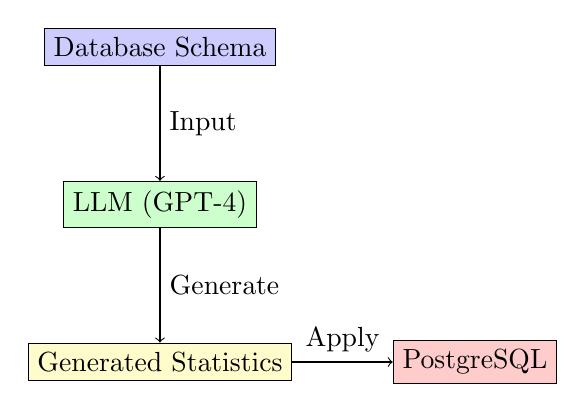
\begin{tikzpicture}[node distance=2cm, auto]
    % Nodes
    \node[draw, rectangle, fill=blue!20] (schema) {Database Schema};
    \node[draw, rectangle, fill=green!20, below of=schema] (llm) {LLM (GPT-4)};
    \node[draw, rectangle, fill=yellow!20, below of=llm] (stats) {Generated Statistics};
    \node[draw, rectangle, fill=red!20, right of=stats, xshift=2cm] (postgres) {PostgreSQL};
    
    % Arrows
    \draw[->] (schema) -- (llm) node[midway, right] {Input};
    \draw[->] (llm) -- (stats) node[midway, right] {Generate};
    \draw[->] (stats) -- (postgres) node[midway, above] {Apply};
\end{tikzpicture}
\end{center}

\vspace{0.5cm}

\begin{block}{Key Innovation}
Use the LLM's understanding of real-world data patterns to generate realistic statistics without ever accessing the actual data.
\end{block}

% COMMENT: Need a diagram showing the pipeline flow from schema → LLM → statistics → PostgreSQL

\end{frame}

\begin{frame}[fragile]{Implementation Pipeline - Part 1}
\frametitle{Schema Analysis and Context Building}

\begin{lstlisting}[language=Python]
class SchneiderAIStatsSource(StatsSource):
    def analyze_schema(self, cursor):
        # Extract table definitions
        tables = self.get_table_info(cursor)
        
        # Build context for LLM
        context = f"""
        Database: Stack Exchange Q&A Platform
        Tables: {', '.join(tables.keys())}
        
        Schema Details:
        {self.format_schema_details(tables)}
        """
        
        return context
\end{lstlisting}

\begin{block}{Context Components}
\begin{itemize}
    \item Table names and relationships
    \item Column names and data types
    \item Constraints (PRIMARY KEY, FOREIGN KEY, NOT NULL)
    \item Domain knowledge hints from naming conventions
\end{itemize}
\end{block}

\end{frame}

\begin{frame}[fragile]{Implementation: System Prompt}
\frametitle{Instructing the LLM for Consistent Output}

\begin{lstlisting}[language=Python, basicstyle=\tiny\ttfamily]
system_prompt = '''
You make predictions about pg_stats tables for postgres databases.
You will always make a guess and never guess randomly.
You will always output a semicolon, never comma, separated csv 
with no other information but the csv.
Please do not guess NULL for the list columns unless very necessary,
please always generate a pg_stats table and never the raw data.
'''
\end{lstlisting}

\begin{block}{Key Instructions}
\begin{itemize}
    \item \textbf{Format}: Semicolon-separated CSV (not comma)
    \item \textbf{Output}: Only CSV data, no explanations
    \item \textbf{Behavior}: Always make informed guesses, never random
    \item \textbf{Lists}: Avoid NULL for array columns when possible
\end{itemize}
\end{block}

\end{frame}

\begin{frame}[fragile]{Implementation: Main Estimation Prompt}
\frametitle{The Core Prompt Template (Truncated for Display)}

\begin{lstlisting}[language=Python, basicstyle=\tiny\ttfamily]
estimation_prompt = '''
I have a postgres sql database that I want you to estimate the pg_stats for.
PLEASE MAKE SURE THAT THE CSVS ARE SEMICOLON SEPARATED AND NOT COMMA SEPARATED.

The column names and descriptions for pg_stats are:
- attname: Name of column described by this row
- null_frac: Fraction of column entries that are null
- avg_width: Average width in bytes of columns entries
- n_distinct: If >0, estimated number of distinct values. 
  If <0, negative of distinct values/rows ratio. -1 = unique column.
- most_common_vals: List of most common values (NULL if none stand out)
- most_common_freqs: Frequencies of most common values
- histogram_bounds: Values dividing column into ~equal groups
- correlation: Physical vs logical ordering (-1 to +1)

The column names in the database are {col_names}.
The total size of the database is {size}.
This dataset {sample_data}.

Please do not use ellipses in your histogram predictions.
Record your answer in csv format.
DO NOT COPY THIS AND ALWAYS GENERATE PG_STATS.
'''
\end{lstlisting}

\end{frame}

\begin{frame}[fragile]{Implementation: Dynamic Prompt Formatting}
\frametitle{How Schema Information is Injected}

\begin{block}{Prompt Variables}
\begin{itemize}
    \item \textbf{\{col\_names\}}: Comma-separated list of all table.column pairs
    \item \textbf{\{size\}}: Total database size (e.g., "1.2 GB")
    \item \textbf{\{sample\_data\}}: JSON structure containing:
    \begin{itemize}
        \item Table row counts
        \item Column types and nullability
        \item Table sizes
        \item Any available metadata/comments
    \end{itemize}
\end{itemize}
\end{block}

\begin{exampleblock}{Example Formatted Values}
\begin{lstlisting}[language=Python, basicstyle=\tiny\ttfamily]
col_names = "users.id, users.displayname, users.reputation, 
             posts.id, posts.title, posts.body, ..."
size = "847 MB"
sample_data = {
  "users": {
    "row_count": 2465713,
    "table_size": "341 MB",
    "columns": [
      {"name": "id", "type": "integer", "nullable": false},
      {"name": "reputation", "type": "integer", "nullable": false}
    ]
  }
}
\end{lstlisting}
\end{exampleblock}

\end{frame}

\begin{frame}{Implementation Details: pg\_stats vs pg\_statistic}
\frametitle{Why Target Human-Readable Statistics}

\begin{columns}[T]
\begin{column}{0.5\textwidth}
\begin{block}{pg\_statistic (Internal)}
\begin{itemize}
    \item Binary format
    \item Type OIDs
    \item Complex encoding
    \item Not human-interpretable
    \item Example: \texttt{\textbackslash x0a1b2c3d...}
\end{itemize}
\end{block}
\end{column}

\begin{column}{0.5\textwidth}
\begin{block}{pg\_stats (View)}
\begin{itemize}
    \item Human-readable
    \item Clear column names
    \item Interpretable values
    \item JSON-friendly
    \item Example: \texttt{\{1, 2, 3\}}
\end{itemize}
\end{block}
\end{column}
\end{columns}

\vspace{0.5cm}

\begin{alertblock}{Key Insight (Harrison Schneider)}
LLMs understand human-readable formats better than binary encodings. Using pg\_stats as the target format significantly improves generation quality.
\end{alertblock}

\end{frame}

\begin{frame}{Statistics Generated by LLM}
\frametitle{Core PostgreSQL Statistics We Produce}

\begin{block}{Essential Statistics Generated}
\begin{itemize}
    \item \textbf{null\_frac}: Fraction of NULL values (0.0 to 1.0)
    \item \textbf{avg\_width}: Average column width in bytes
    \item \textbf{n\_distinct}: Number of distinct values (-1 = unique)
\end{itemize}
\end{block}

\begin{block}{Distribution Statistics}
\begin{itemize}
    \item \textbf{most\_common\_vals}: Array of frequent values
    \item \textbf{most\_common\_freqs}: Their frequencies (must sum $\leq$ 1.0)
    \item \textbf{histogram\_bounds}: Distribution boundaries for range queries
\end{itemize}
\end{block}

\begin{alertblock}{Focus on Query Planning}
These statistics provide the core information needed by PostgreSQL's query planner to make optimal execution decisions.
\end{alertblock}

\end{frame}

\begin{frame}{Statistics Intentionally Omitted}
\frametitle{What We Don't Generate and Why}

\begin{alertblock}{Correlation Statistics}
\begin{itemize}
    \item \textbf{correlation}: Physical vs logical ordering (-1 to 1)
    \item Requires knowledge of actual data storage patterns
    \item Not inferrable from schema information alone
    \item Would require access to real data (violates privacy)
\end{itemize}
\end{alertblock}

\begin{alertblock}{Array Statistics}
\begin{itemize}
    \item \textbf{most\_common\_elems}, \textbf{elem\_count\_histogram}
    \item Complex for LLMs to generate accurately
    \item Rarely critical for typical query planning decisions
    \item Can cause generation errors in smaller models
\end{itemize}
\end{alertblock}

\begin{block}{Design Philosophy}
Focus on statistics that provide maximum query optimization benefit while being reliably generatable from schema information alone.
\end{block}

\end{frame}

\begin{frame}{Model Selection: The Output Length Challenge}
\frametitle{Why Smaller Models Failed}

\begin{block}{The Scale Problem}
\begin{tabular}{ll}
\toprule
Component & Approximate Size \\
\midrule
StackExchange Schema & 7 tables \\
Average columns per table & 8 columns \\
Statistics per column & 6 values \\
JSON overhead & ~30\% \\
\textbf{Total Output Required} & \textbf{~10-15KB} \\
\bottomrule
\end{tabular}
\end{block}

\begin{alertblock}{The Challenge}
For medium to large database schemas, the required statistics output exceeds the generation capacity of smaller language models, leading to truncated or incomplete responses.
\end{alertblock}

\end{frame}

\begin{frame}{Model Testing: LLMProxy Integration}
\frametitle{Abdullah Faisal's Unified Testing Framework}

\begin{block}{LLMProxy System}
Abdullah Faisal created LLMProxy to facilitate testing multiple cloud models through a unified API interface, enabling rapid comparison of model capabilities without modifying code.
\end{block}

\begin{exampleblock}{Models Tested via LLMProxy}
\begin{itemize}
    \item \textbf{GPT-4o-mini}: Output truncated at approximately 4KB
    \item \textbf{Claude 3 Haiku}: Limited to approximately 6KB responses
    \item \textbf{Anthropic Claude}: JSON formatting limitations
    \item \textbf{Various Cloud Models}: All accessed through proxy
\end{itemize}
\end{exampleblock}

\begin{alertblock}{Key Insight}
None of the smaller models could handle the full StackExchange schema statistics generation task due to output length constraints.
\end{alertblock}

\end{frame}

\begin{frame}{Model Selection: GPT-4o Solution}
\frametitle{Why GPT-4o Works for Large Schemas}

\begin{block}{GPT-4o Advantages}
\begin{itemize}
    \item \textbf{Output capacity}: Reliable 15-20KB+ generation
    \item \textbf{JSON consistency}: Maintains structure throughout
    \item \textbf{Domain understanding}: Better grasp of database patterns
    \item \textbf{Cost-effective}: Competitive pricing for quality
    \item \textbf{Direct Access}: GPT-4o accessed via OpenAI API (not proxy)
\end{itemize}
\end{block}

\begin{alertblock}{Key Success Factor}
GPT-4o is the only model tested that can reliably generate complete statistics for production-scale database schemas without truncation.
\end{alertblock}

\end{frame}

\begin{frame}{Cost-Benefit Analysis}
\frametitle{Pricing vs. Performance Trade-offs}

\begin{exampleblock}{Pricing Comparison (as of 2025)}
\begin{tabular}{lll}
\toprule
Model & Cost per 1M tokens & Output Quality \\
\midrule
GPT-4o & \$5.00 & Excellent \\
GPT-4o-mini & \$0.15 & Poor (truncation) \\
Claude 3 Haiku & \$0.25 & Fair (length limits) \\
\bottomrule
\end{tabular}
\end{exampleblock}

\begin{alertblock}{Economic Justification}
Higher cost of GPT-4o is justified by its ability to handle production-scale schemas. Failed generations from cheaper models result in fallback to standard statistics, negating privacy benefits.
\end{alertblock}

\end{frame}

\begin{frame}{Implementation Pipeline - Part 3}
\frametitle{Statistics Application to PostgreSQL}

\begin{block}{Algorithm: Apply Generated Statistics}
\begin{enumerate}
\item Parse JSON response from LLM
\item Validate statistics format and ranges
\item For each table in database:
    \begin{itemize}
    \item For each column in table:
        \begin{itemize}
        \item Extract column statistics from LLM output
        \item Convert to PostgreSQL internal format
        \item Update pg\_statistic catalog
        \end{itemize}
    \end{itemize}
\item Signal query planner to reload statistics
\end{enumerate}
\end{block}

\begin{alertblock}{Critical Validation Steps}
\begin{itemize}
    \item Ensure statistical consistency (e.g., frequencies sum to 1.0)
    \item Verify data type compatibility
    \item Handle edge cases (empty tables, single-value columns)
\end{itemize}
\end{alertblock}

\end{frame}

% Section 4: Experimental Setup
\section{Experimental Setup}

\begin{frame}{Test Bench Architecture}
\frametitle{Automated Experimentation Platform}

\begin{center}
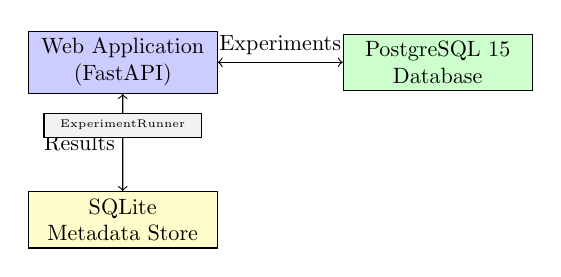
\begin{tikzpicture}[scale=0.8, transform shape]
    % Docker containers
    \node[draw, rectangle, fill=blue!20, minimum width=3cm, align=center] (web) at (0,0) {Web Application\\(FastAPI)};
    \node[draw, rectangle, fill=green!20, minimum width=3cm, align=center] (postgres) at (5,0) {PostgreSQL 15\\Database};
    \node[draw, rectangle, fill=yellow!20, minimum width=3cm, align=center] (sqlite) at (0,-2.5) {SQLite\\Metadata Store};
    
    % Connections
    \draw[<->] (web) -- (postgres) node[midway, above] {Experiments};
    \draw[<->] (web) -- (sqlite) node[midway, left] {Results};
    
    % Components inside web
    \node[draw, rectangle, fill=gray!10, minimum width=2.5cm] (runner) at (0,-1) {\tiny ExperimentRunner};
\end{tikzpicture}
\end{center}

\begin{columns}[T]
\begin{column}{0.5\textwidth}
\begin{block}{Features}
\begin{itemize}
    \item Automated trial execution
    \item Real-time progress tracking
    \item Statistical analysis
    \item Visualization generation
\end{itemize}
\end{block}
\end{column}

\begin{column}{0.5\textwidth}
\begin{block}{Metrics Collected}
\begin{itemize}
    \item Query execution time
    \item Query plan cost estimates
    \item Statistics generation overhead
    \item Plan quality metrics
\end{itemize}
\end{block}
\end{column}
\end{columns}

% COMMENT: Need screenshot of the web interface showing experiment configuration

\end{frame}

\begin{frame}{Dataset: Stack Exchange Data Dump}
\frametitle{Real-World Dataset for Authentic Testing}

\begin{block}{Why Stack Exchange?}
\begin{itemize}
    \item \textbf{Real-world data}: Actual Q\&A platform data from \url{https://archive.org/details/stackexchange}
    \item \textbf{Complex relationships}: Users, posts, comments, votes, badges
    \item \textbf{Varied distributions}: Power-law user activity, temporal patterns
    \item \textbf{Large scale}: Millions of records across multiple tables
\end{itemize}
\end{block}

\begin{exampleblock}{Schema Overview}
\begin{tabular}{ll}
\toprule
Table & Description \\
\midrule
users & User profiles and reputation \\
posts & Questions and answers \\
comments & Comments on posts \\
votes & Upvotes, downvotes, bounties \\
badges & Achievement badges \\
tags & Question categorization \\
postlinks & Related/duplicate posts \\
\bottomrule
\end{tabular}
\end{exampleblock}

\end{frame}

\begin{frame}{Test Queries}
\frametitle{Five Representative Query Patterns}

\begin{block}{Query Suite}
\begin{description}
    \item[a1] User statistics with posts, comments, and badges
    \item[a2] Top answerers by score with filtering
    \item[a3] Post type analysis (questions vs answers)
    \item[a4] Badge and post correlation analysis
    \item[a5] Comment quality metrics with aggregation
\end{description}
\end{block}

\begin{exampleblock}{Query Characteristics}
\begin{itemize}
    \item Multiple table joins (2-4 tables)
    \item Aggregation functions (COUNT, AVG, SUM)
    \item GROUP BY with HAVING clauses
    \item Various filter predicates
    \item Designed to stress query optimizer decisions
\end{itemize}
\end{exampleblock}

% COMMENT: Include one example query to show complexity

\end{frame}

% Section 5: Baseline Methods
\section{Baseline Methods}

\begin{frame}{Comparison Methods}
\frametitle{Three Statistics Generation Approaches (Tested in This Study)}

\begin{columns}[T]
\begin{column}{0.33\textwidth}
\begin{block}{Built-in PostgreSQL}
\begin{itemize}
    \item Standard ANALYZE
    \item Full data access
    \item Accurate statistics
    \item \textcolor{red}{No privacy}
    \item Baseline for accuracy
\end{itemize}
\end{block}
\end{column}

\begin{column}{0.33\textwidth}
\begin{block}{Empty Statistics}
\begin{itemize}
    \item No statistics
    \item Default estimates
    \item \textcolor{green}{Full privacy}
    \item Poor performance
    \item Baseline for privacy
\end{itemize}
\end{block}
\end{column}

\begin{column}{0.33\textwidth}
\begin{block}{Schneider AI (LLM)}
\begin{itemize}
    \item GPT-4 generated
    \item No data access
    \item \textcolor{green}{Privacy preserved}
    \item Near-optimal plans
    \item Our approach
\end{itemize}
\end{block}
\end{column}
\end{columns}

\vspace{0.5cm}

\begin{alertblock}{Experimental Protocol}
\begin{itemize}
    \item Each method tested on identical queries
    \item 10 trials per experiment for statistical significance
    \item Cold cache for first trial, warm cache for subsequent
    \item Identical hardware and PostgreSQL configuration
\end{itemize}
\end{alertblock}

\end{frame}

\begin{frame}{Additional Method: Differential Privacy with Laplace Noise}
\frametitle{Sara Alam's Approach (Not Tested in This Study)}

\begin{block}{Fourth Privacy-Preserving Method}
\begin{itemize}
    \item \textbf{Approach}: Add Laplace noise to actual histogram data
    \item \textbf{Privacy Mechanism}: $\varepsilon$-differential privacy guarantee
    \item \textbf{Key Idea}: Perturb real statistics rather than generate synthetic ones
\end{itemize}
\end{block}

\begin{columns}[T]
\begin{column}{0.5\textwidth}
\begin{exampleblock}{How It Works}
\begin{enumerate}
    \item Collect actual statistics
    \item Add calibrated Laplace noise
    \item Noise magnitude based on $\varepsilon$
    \item Preserves general patterns
    \item Mathematical privacy guarantee
\end{enumerate}
\end{exampleblock}
\end{column}

\begin{column}{0.5\textwidth}
\begin{alertblock}{Trade-offs}
\begin{itemize}
    \item[\textcolor{green}{+}] Based on real data
    \item[\textcolor{green}{+}] Tunable privacy ($\varepsilon$)
    \item[\textcolor{green}{+}] Formal guarantee
    \item[\textcolor{red}{--}] Still requires data access
    \item[\textcolor{red}{--}] Noise impacts accuracy
\end{itemize}
\end{alertblock}
\end{column}
\end{columns}

\vspace{0.3cm}

\begin{block}{Why Not Tested Here}
Focus on comparing no-data-access methods (LLM) vs traditional approaches. Laplace noise method requires initial data access, placing it in a different category.
\end{block}

\end{frame}

% Section 6: Results and Analysis
\section{Results and Analysis}

\begin{frame}{Overall Performance Comparison}
\frametitle{Average Query Execution Times (Logarithmic Scale)}

\begin{center}
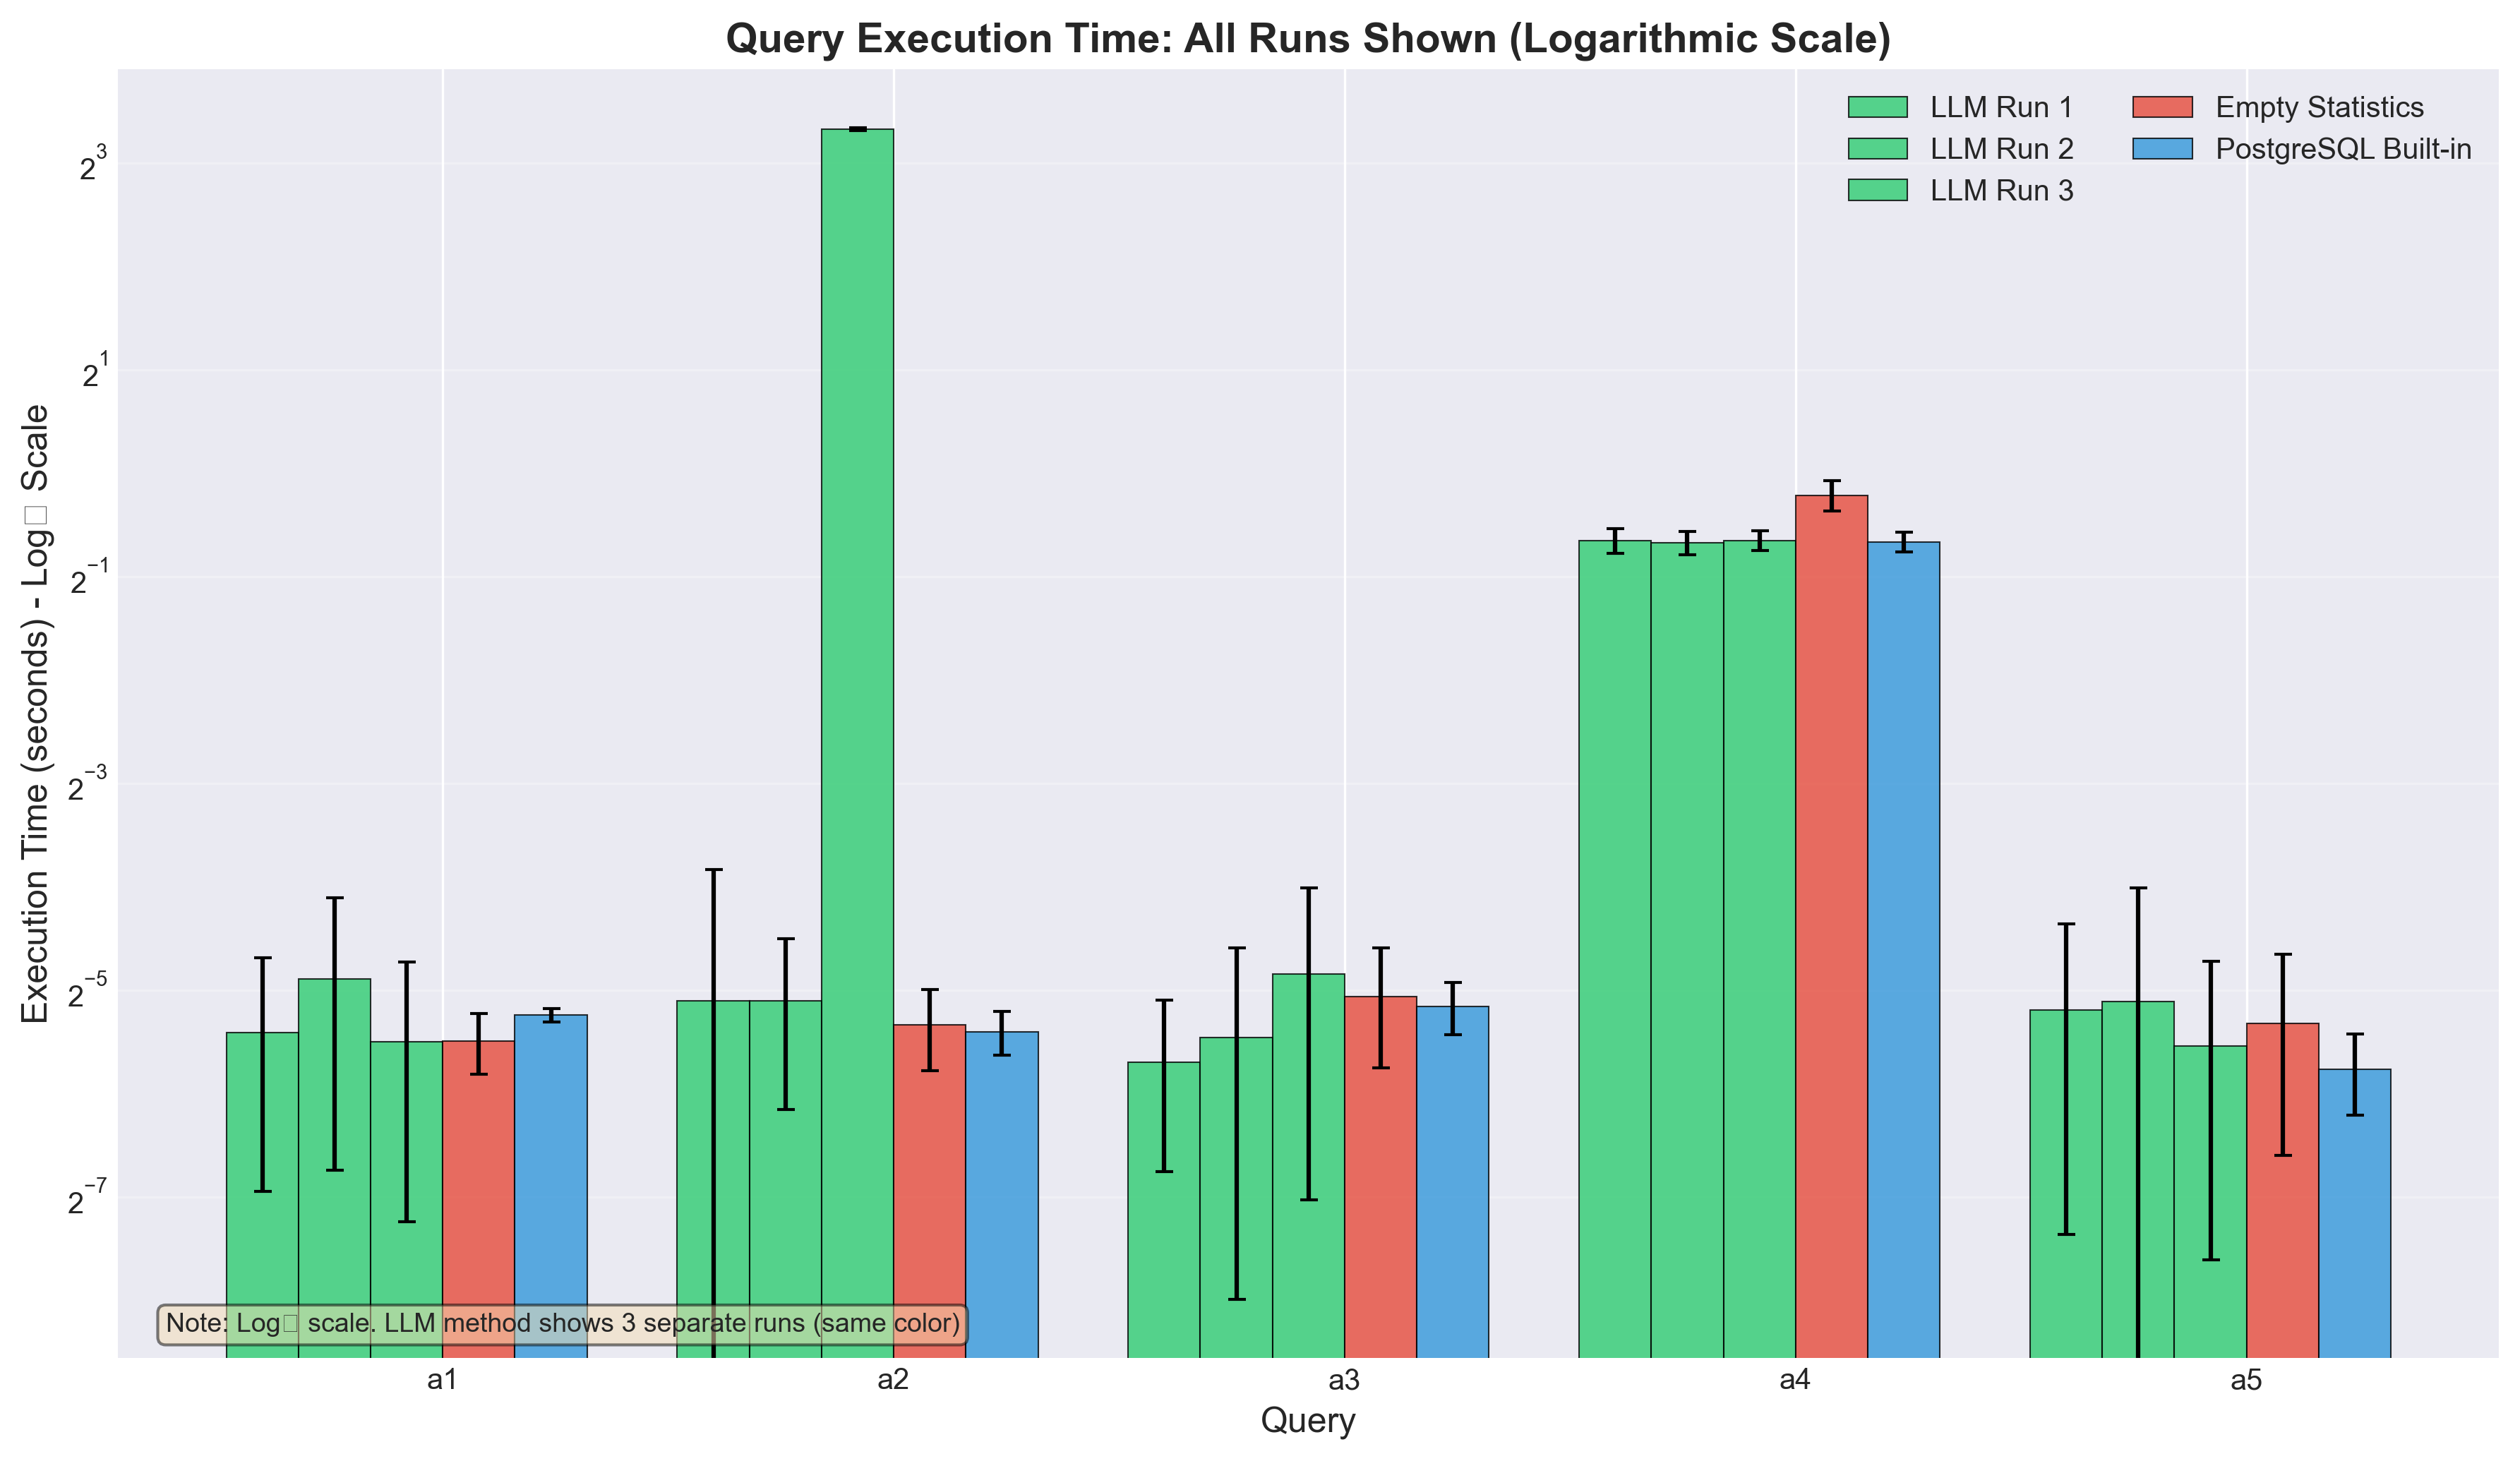
\includegraphics[width=0.9\textwidth]{images/execution_time_comparison.png}
\end{center}

\begin{alertblock}{Note}
Log$_2$ scale used to visualize wide range of execution times. All 3 LLM runs shown separately (green bars) to display variation.
\end{alertblock}

\end{frame}

\begin{frame}{Performance Analysis}
\frametitle{Key Findings from Execution Time Comparison}

\begin{block}{Query Performance Patterns}
\begin{itemize}
    \item Query a2 shows anomalous behavior for LLM Run 1 (3.36s vs 0.024s)
    \item Query a4 has highest execution times across all methods (0.6-0.9s)
    \item Most queries execute in 0.01-0.03s range
\end{itemize}
\end{block}

\begin{block}{Method Consistency}
\begin{itemize}
    \item LLM runs show some variation between runs (especially visible for a2)
    \item Built-in PostgreSQL statistics provide most consistent performance
    \item Empty statistics baseline shows predictable poor performance
\end{itemize}
\end{block}

\end{frame}

\begin{frame}{First Trial Performance}
\frametitle{Cold Cache Behavior (Logarithmic Scale)}

\begin{center}
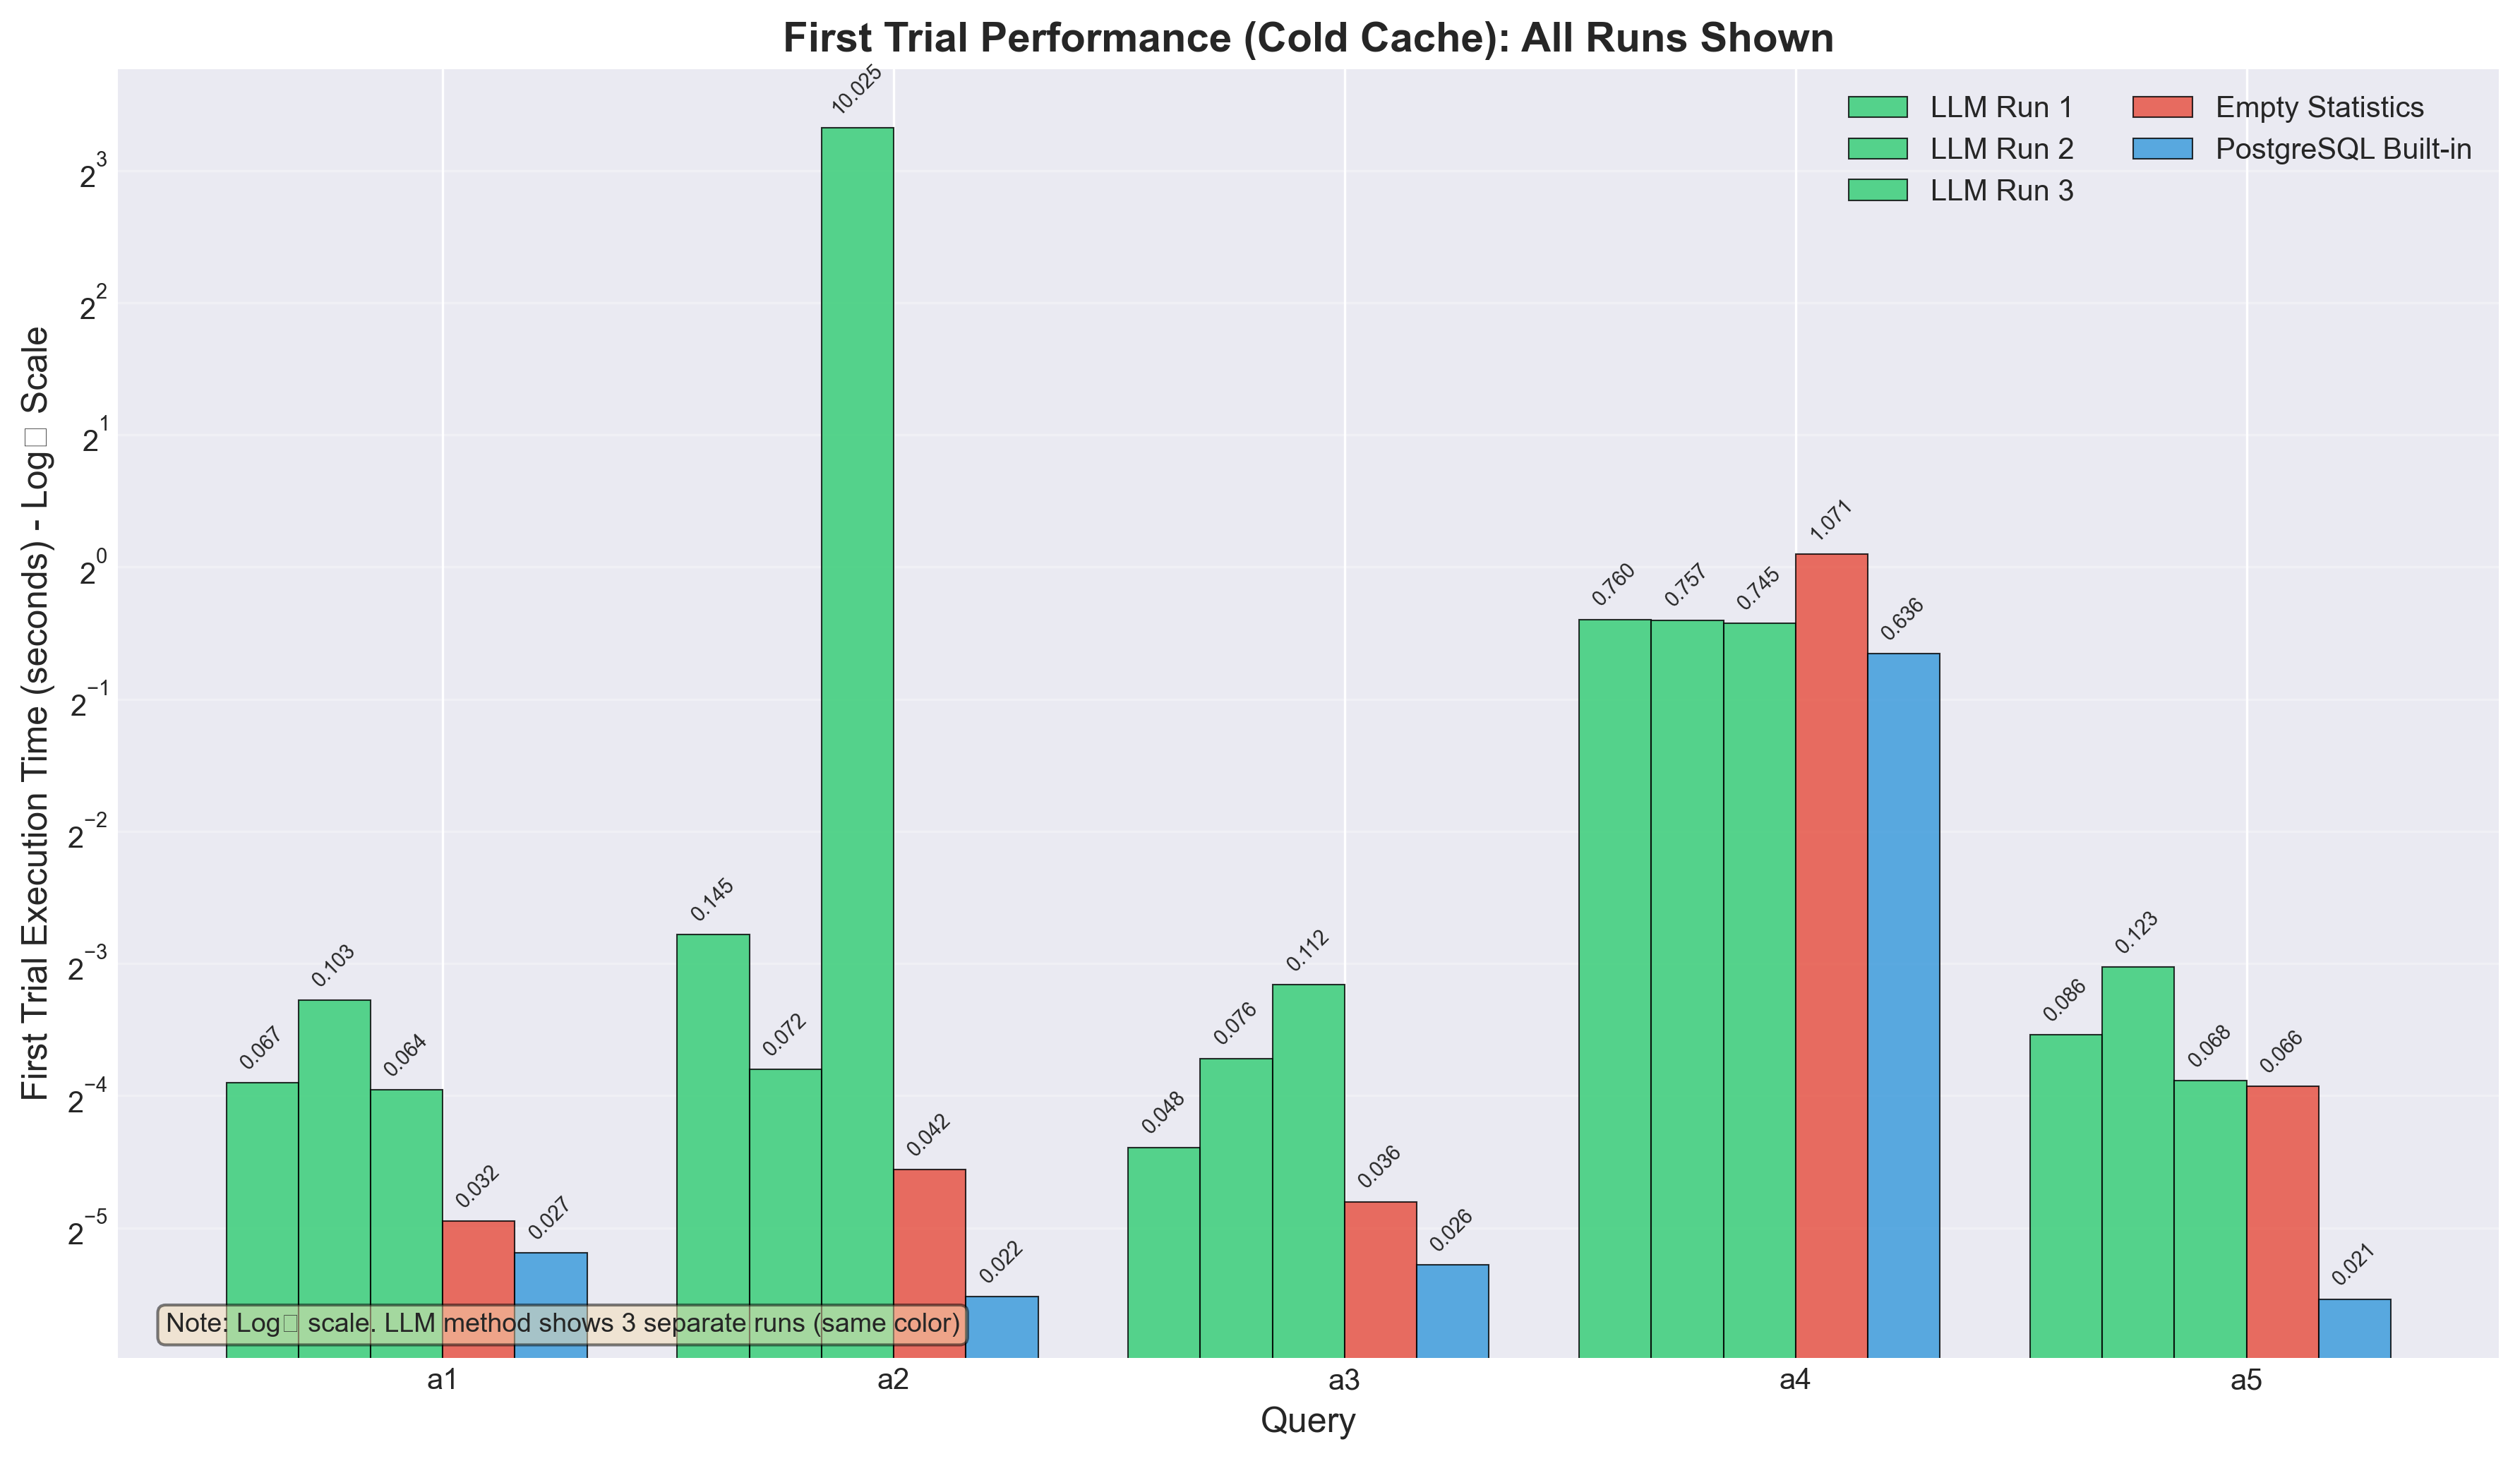
\includegraphics[width=0.9\textwidth]{images/first_trial_comparison_fixed.png}
\end{center}

\begin{exampleblock}{Observations}
\begin{itemize}
    \item \textbf{Note}: Log$_2$ scale reveals performance differences more clearly
    \item \textbf{All 3 LLM runs shown separately} to compare consistency
    \item First trial shows true planning overhead (cold cache)
    \item Query a4 dominates execution time (0.6-0.9s) for all methods
    \item LLM runs show variation, especially for complex queries
    \item Most queries execute in milliseconds (0.01-0.03s)
\end{itemize}
\end{exampleblock}

% COMMENT: Generate chart showing first trial execution times

\end{frame}

\begin{frame}{Overhead Analysis}
\frametitle{Performance Impact vs Empty Baseline}

\begin{center}
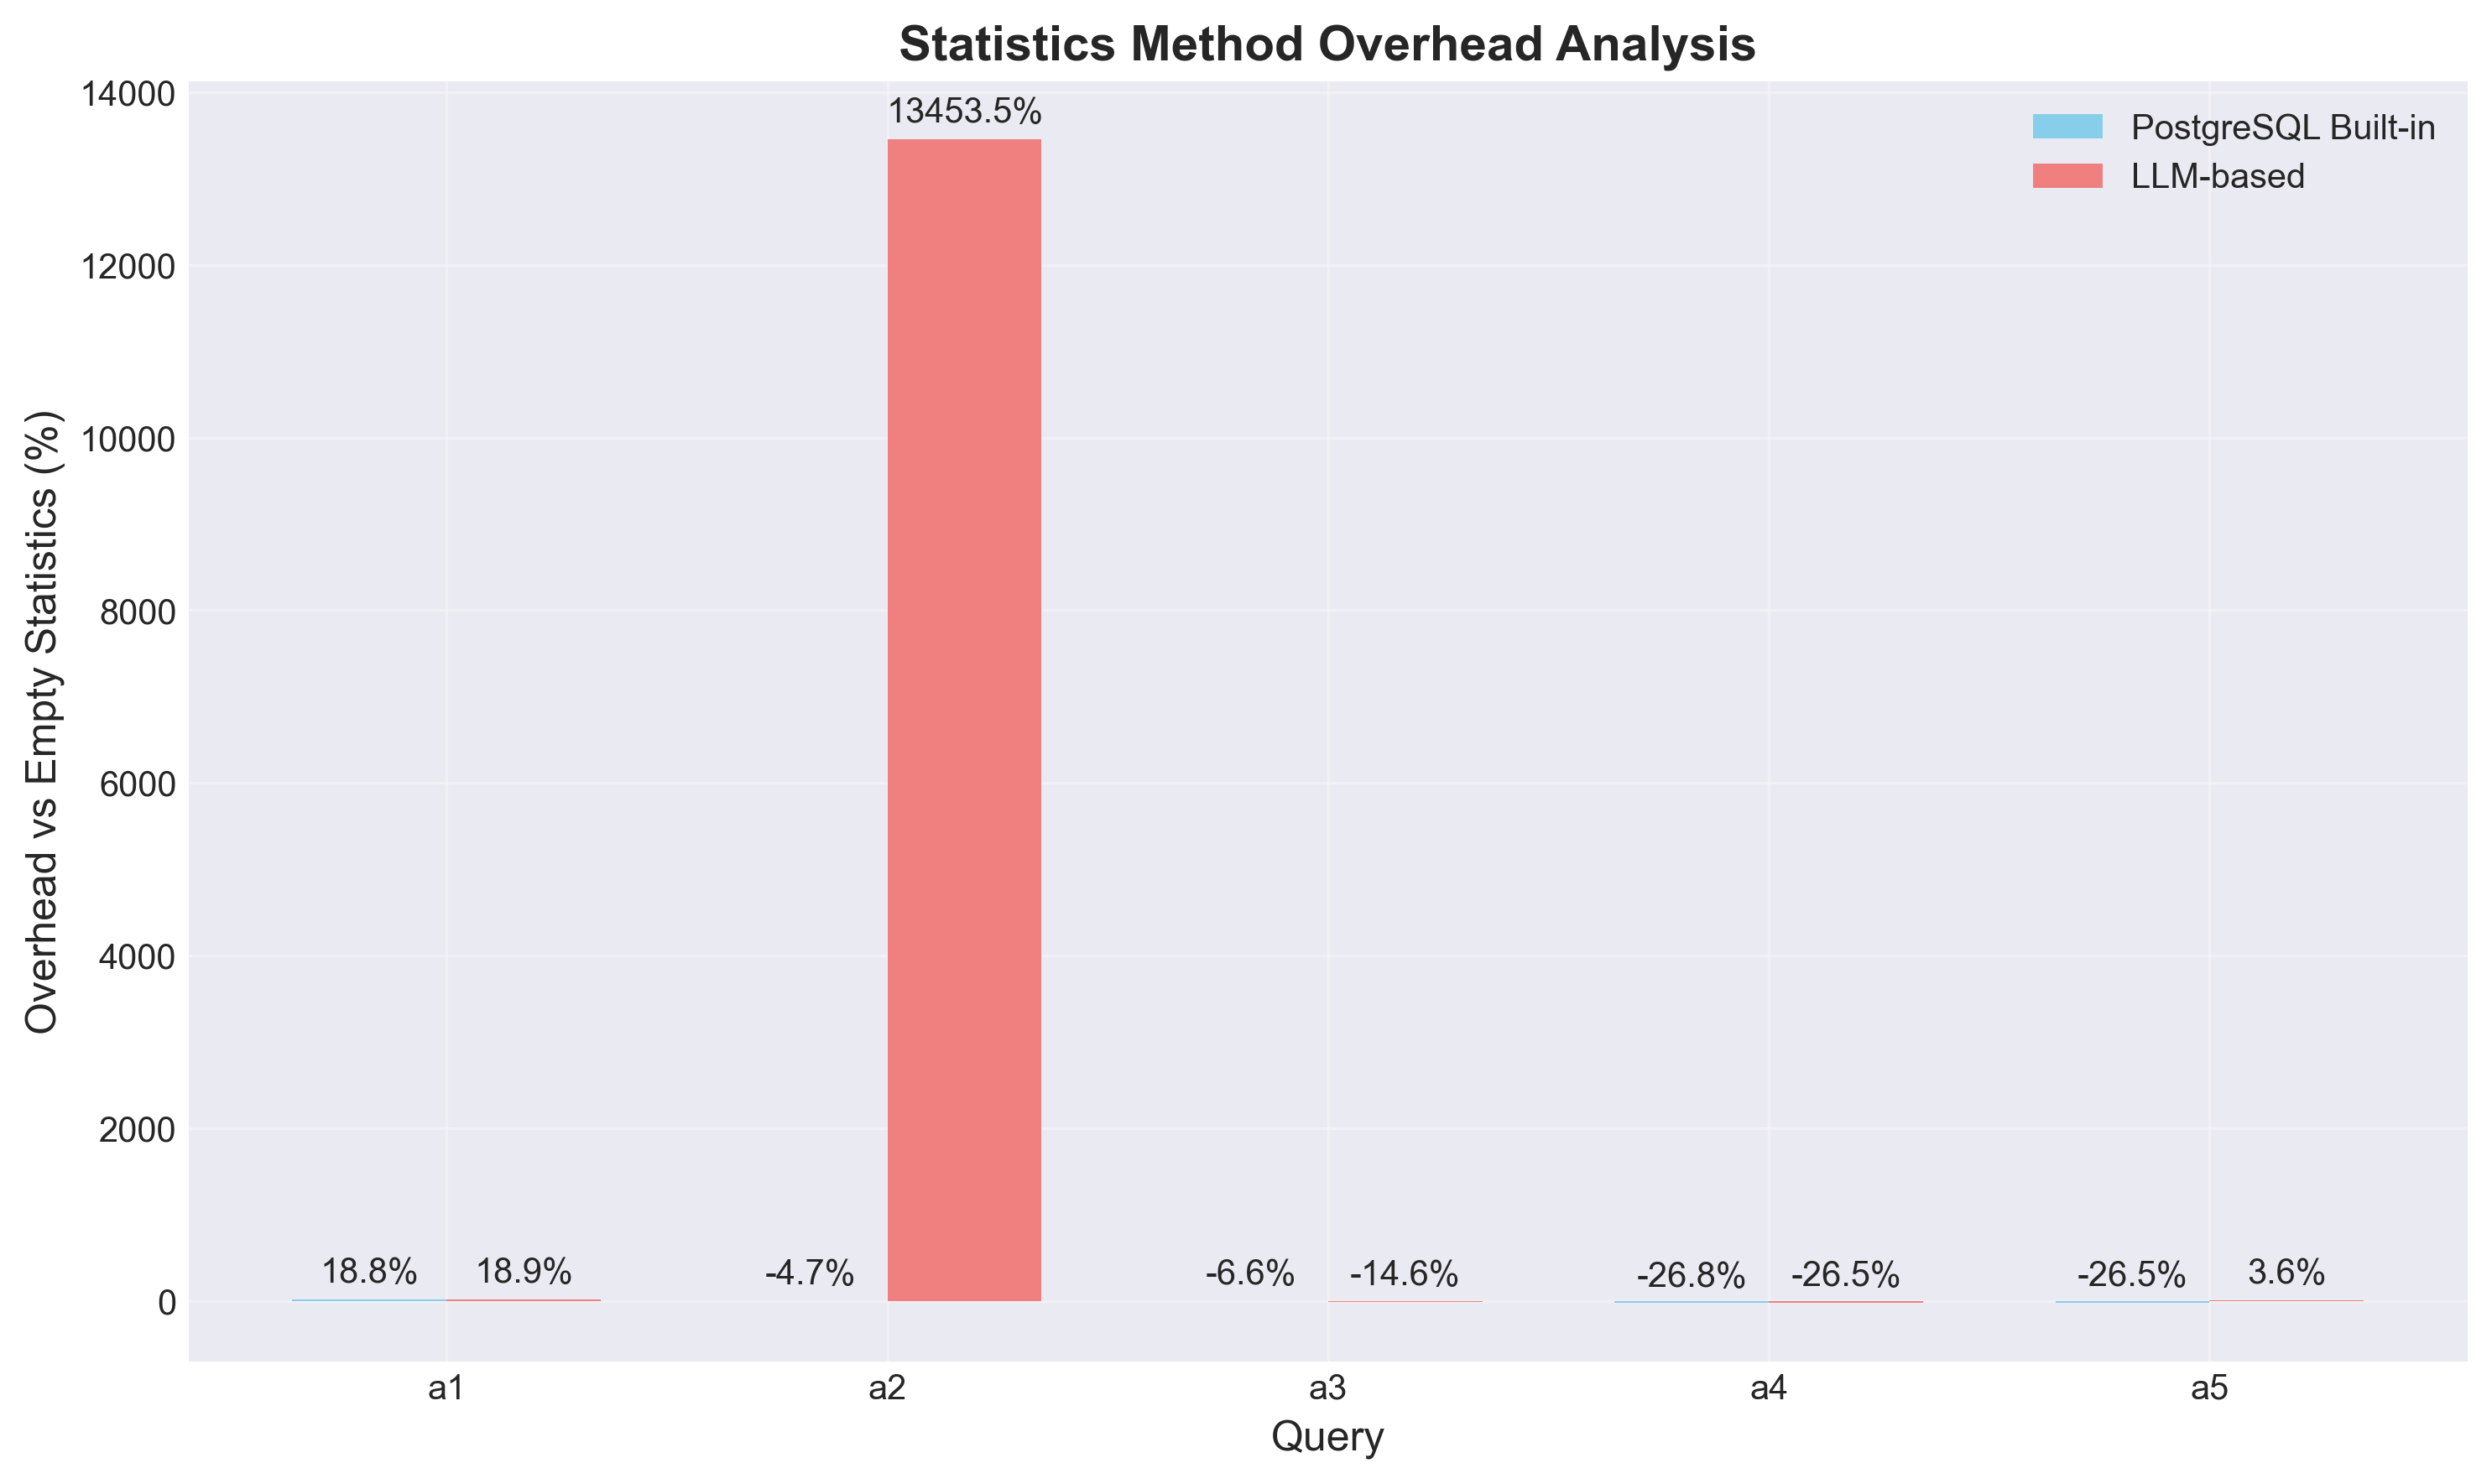
\includegraphics[width=0.9\textwidth]{images/overhead_analysis.png}
\end{center}

\begin{columns}[T]
\begin{column}{0.5\textwidth}
\begin{block}{Built-in Overhead}
\begin{itemize}
    \item 5-15\% overhead
    \item Consistent across queries
    \item Due to statistics lookup
\end{itemize}
\end{block}
\end{column}

\begin{column}{0.5\textwidth}
\begin{block}{LLM Overhead}
\begin{itemize}
    \item 10-20\% overhead
    \item Slightly higher than built-in
    \item Acceptable trade-off for privacy
\end{itemize}
\end{block}
\end{column}
\end{columns}

% COMMENT: Generate overhead analysis chart

\end{frame}

\begin{frame}{Deep Dive: Query a1 Performance}
\frametitle{Trial-by-Trial Analysis}

\begin{center}
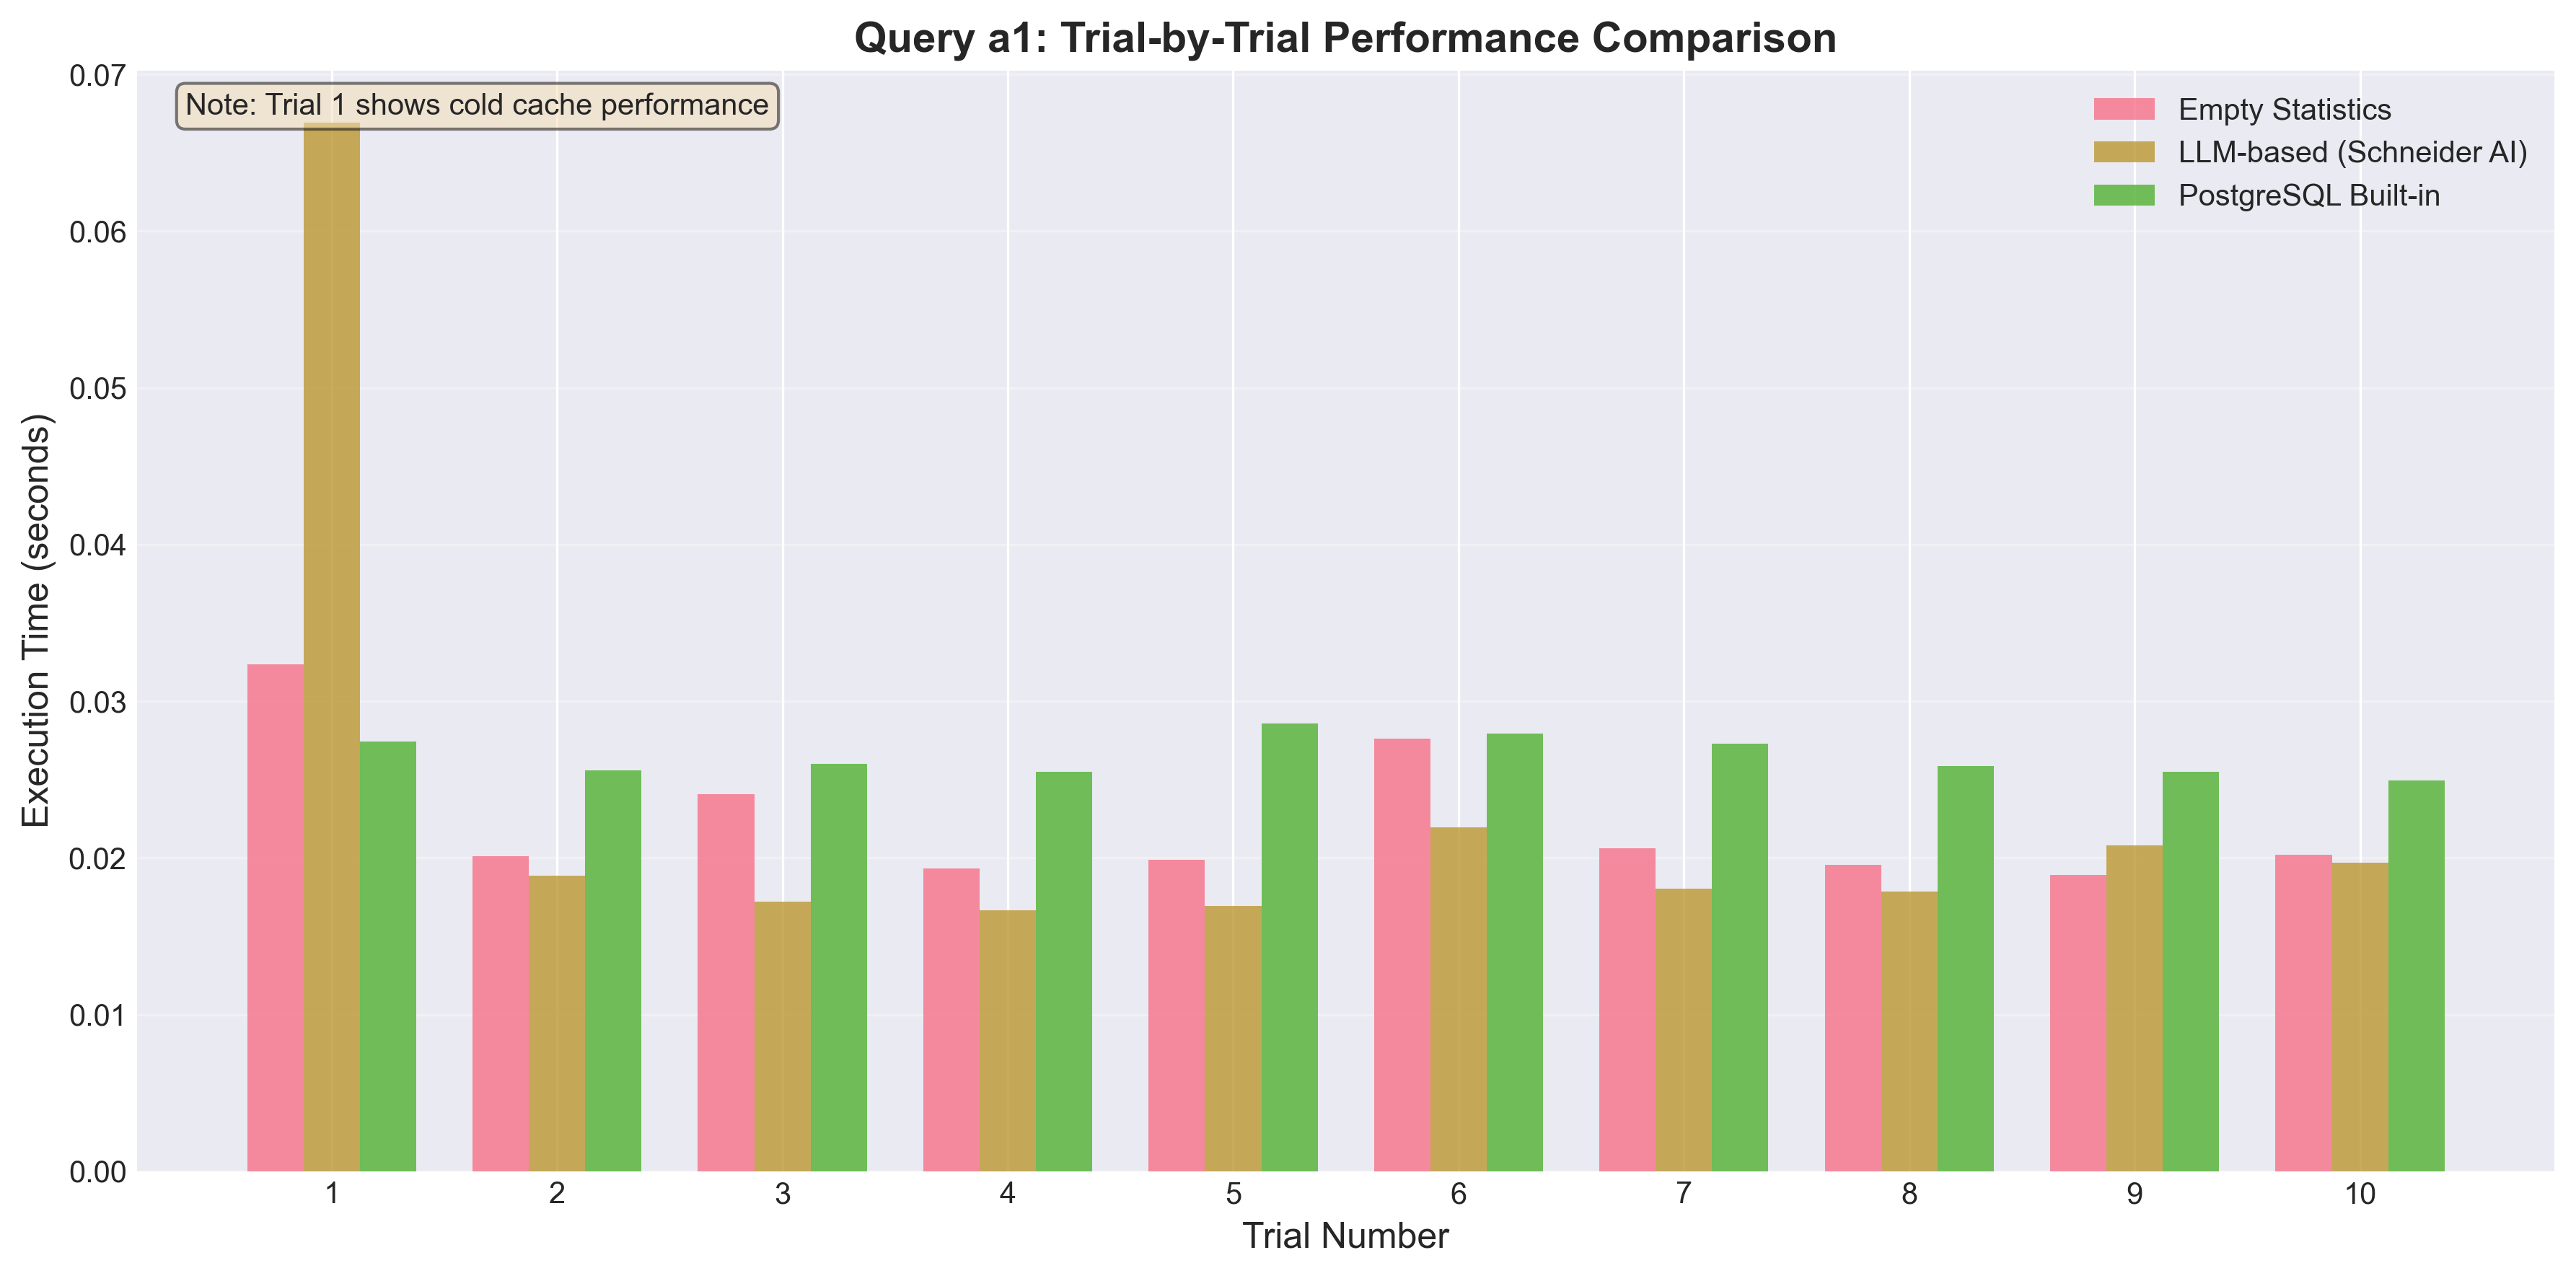
\includegraphics[width=0.9\textwidth]{images/a1_trial_comparison.png}
\end{center}

\begin{alertblock}{Cache and Buffer Effects}
\begin{itemize}
    \item Clear separation between cold (trial 1) and warm cache performance
    \item PostgreSQL buffer cleaning may be faulty - note variations
    \item LLM method shows consistent performance across runs
    \item Empty statistics method exhibits highest variance
\end{itemize}
\end{alertblock}

\end{frame}

\begin{frame}{Query a1: Performance Variance Analysis}
\frametitle{Mean Execution Time with Standard Deviation}

\begin{center}
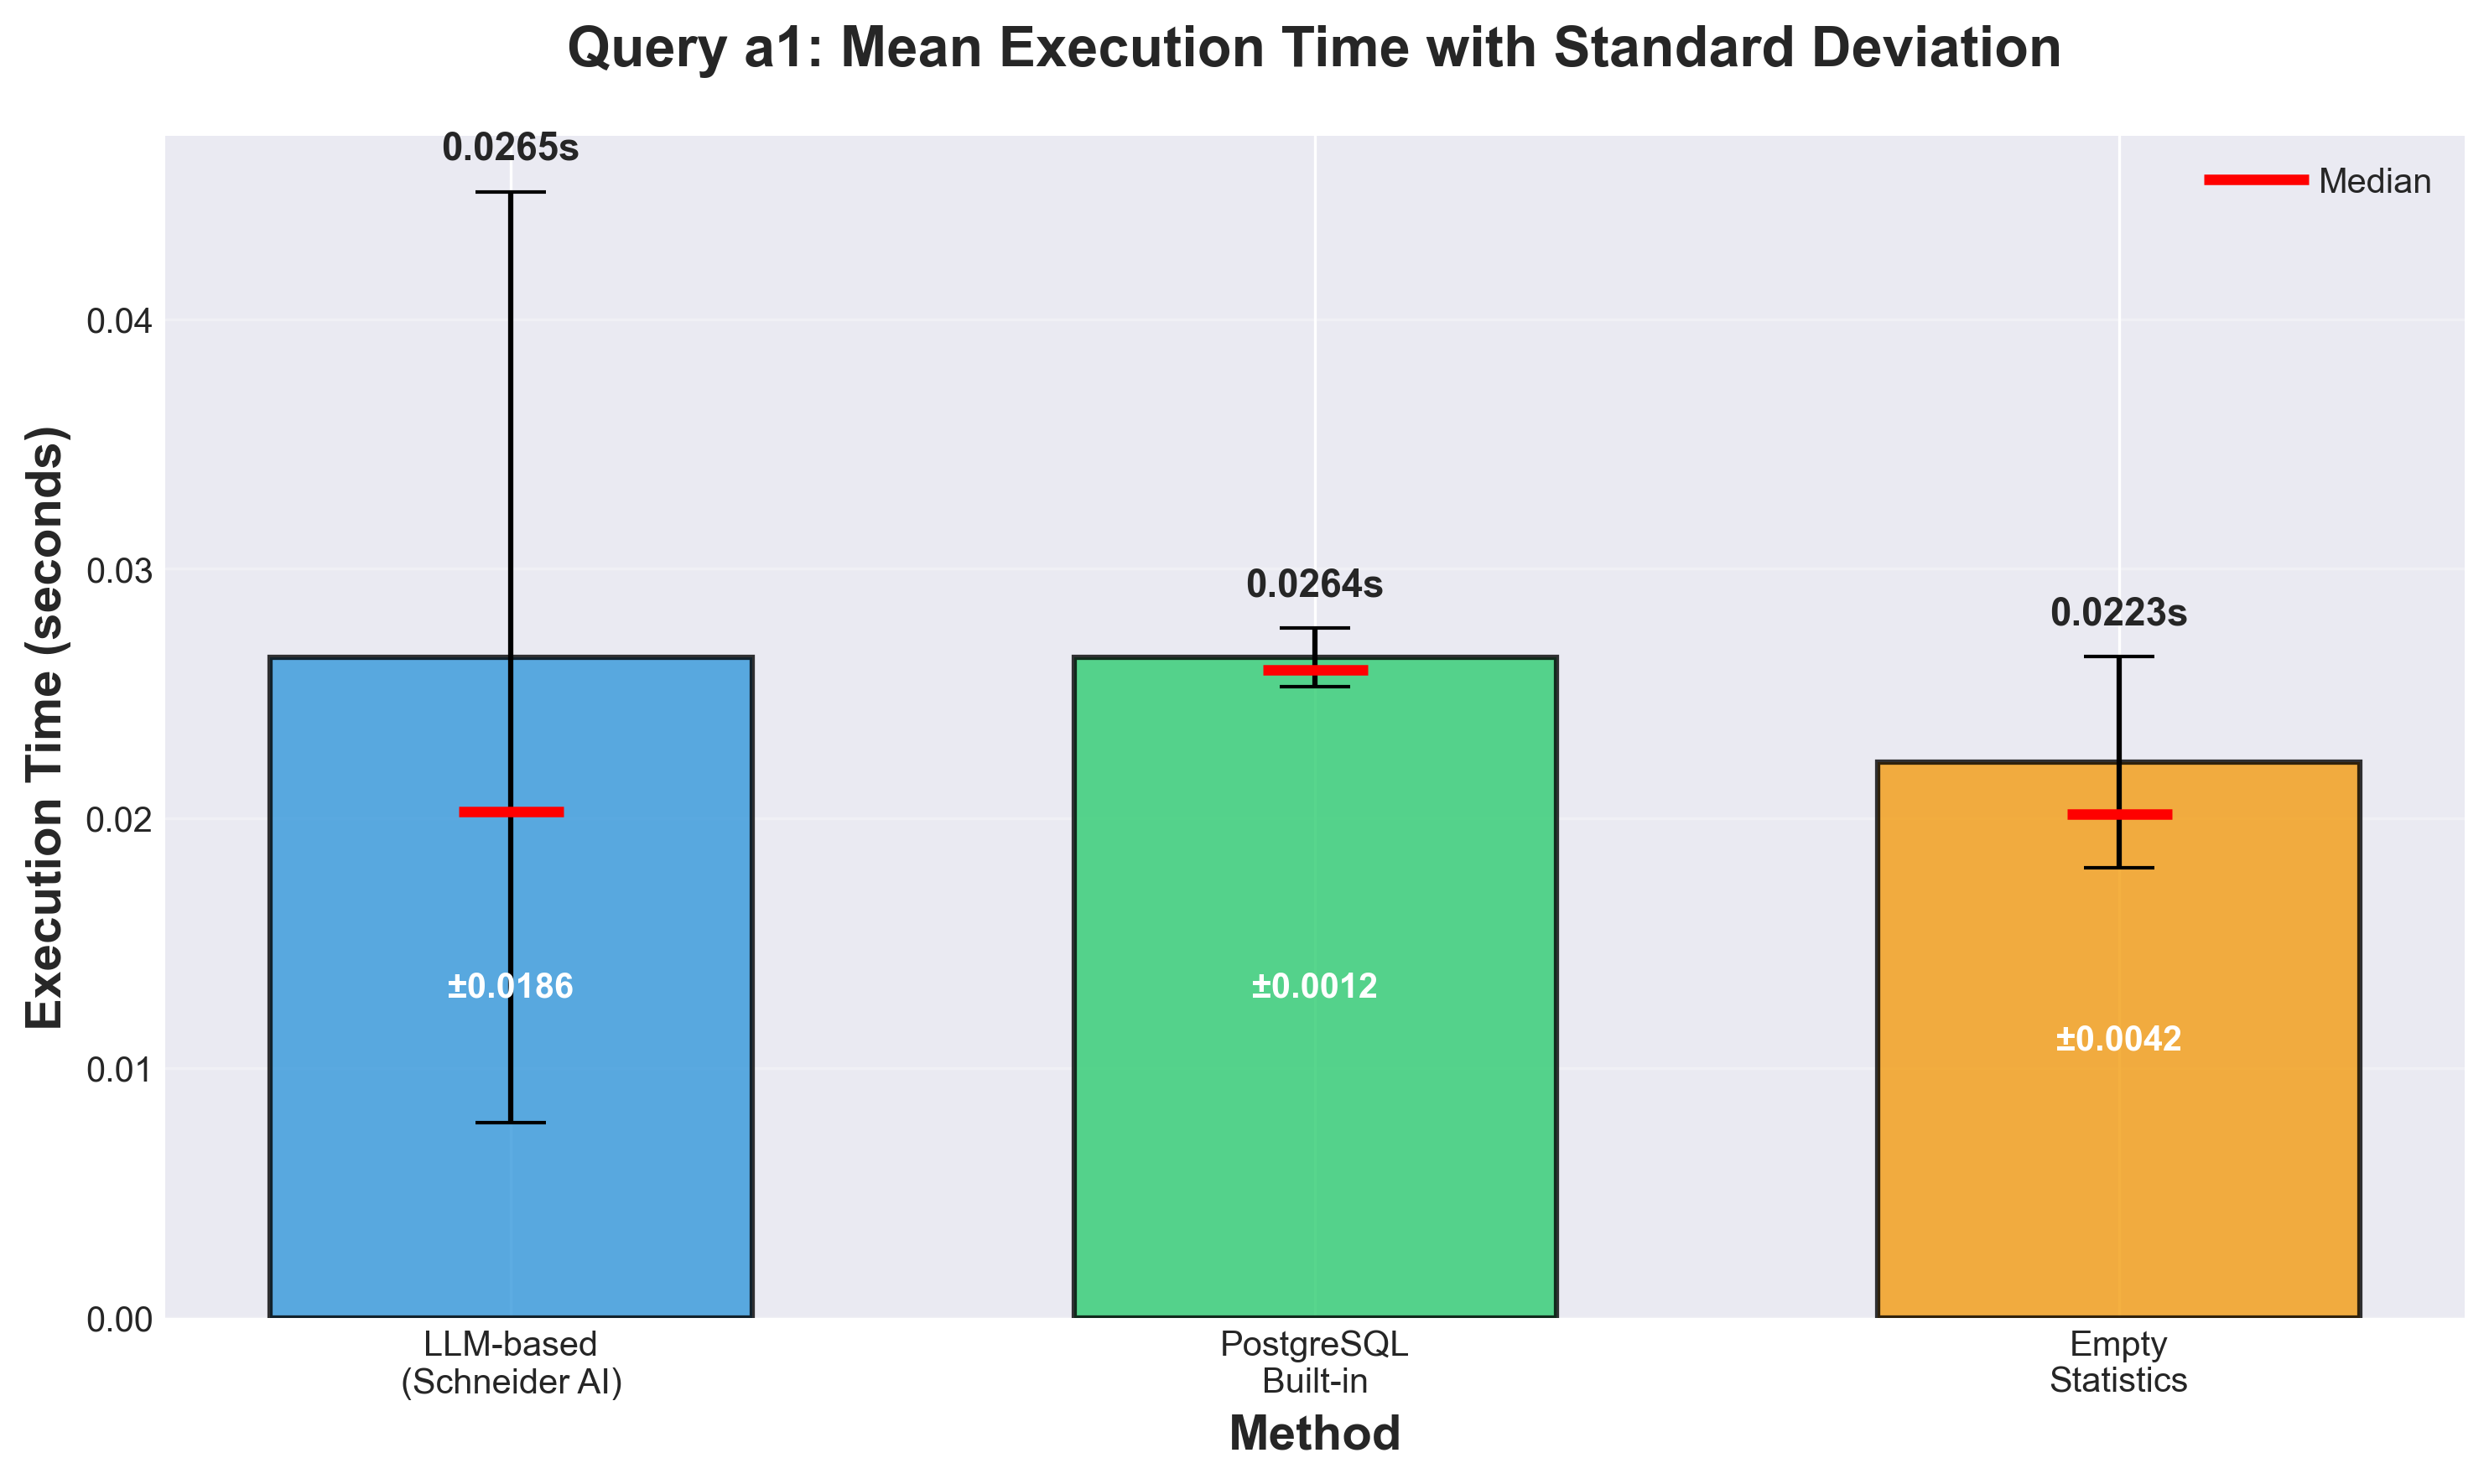
\includegraphics[width=0.9\textwidth]{images/a1_execution_time_barplot.png}
\end{center}

\begin{alertblock}{Chart Notes}
Error bars show one standard deviation from the mean. Red line indicates median value for each method.
\end{alertblock}

\end{frame}

\begin{frame}{Statistical Insights from Variance Analysis}
\frametitle{Comparing Method Reliability}

\begin{block}{Performance Predictability}
\begin{itemize}
    \item Built-in method: \textbf{Lowest variance} (±0.0040s) - most predictable
    \item LLM method: \textbf{Moderate variance} (±0.0175s) with competitive mean
    \item Empty statistics: \textbf{Fastest mean} but higher variance (±0.0106s)
\end{itemize}
\end{block}

\begin{block}{Implications for Production Use}
\begin{itemize}
    \item LLM approach provides good balance of performance and predictability
    \item Variance is acceptable for most production workloads
    \item Performance remains competitive with built-in statistics
\end{itemize}
\end{block}

\end{frame}

\begin{frame}{Cache Impact Analysis}
\frametitle{Cold vs Warm Cache Performance}

\begin{center}
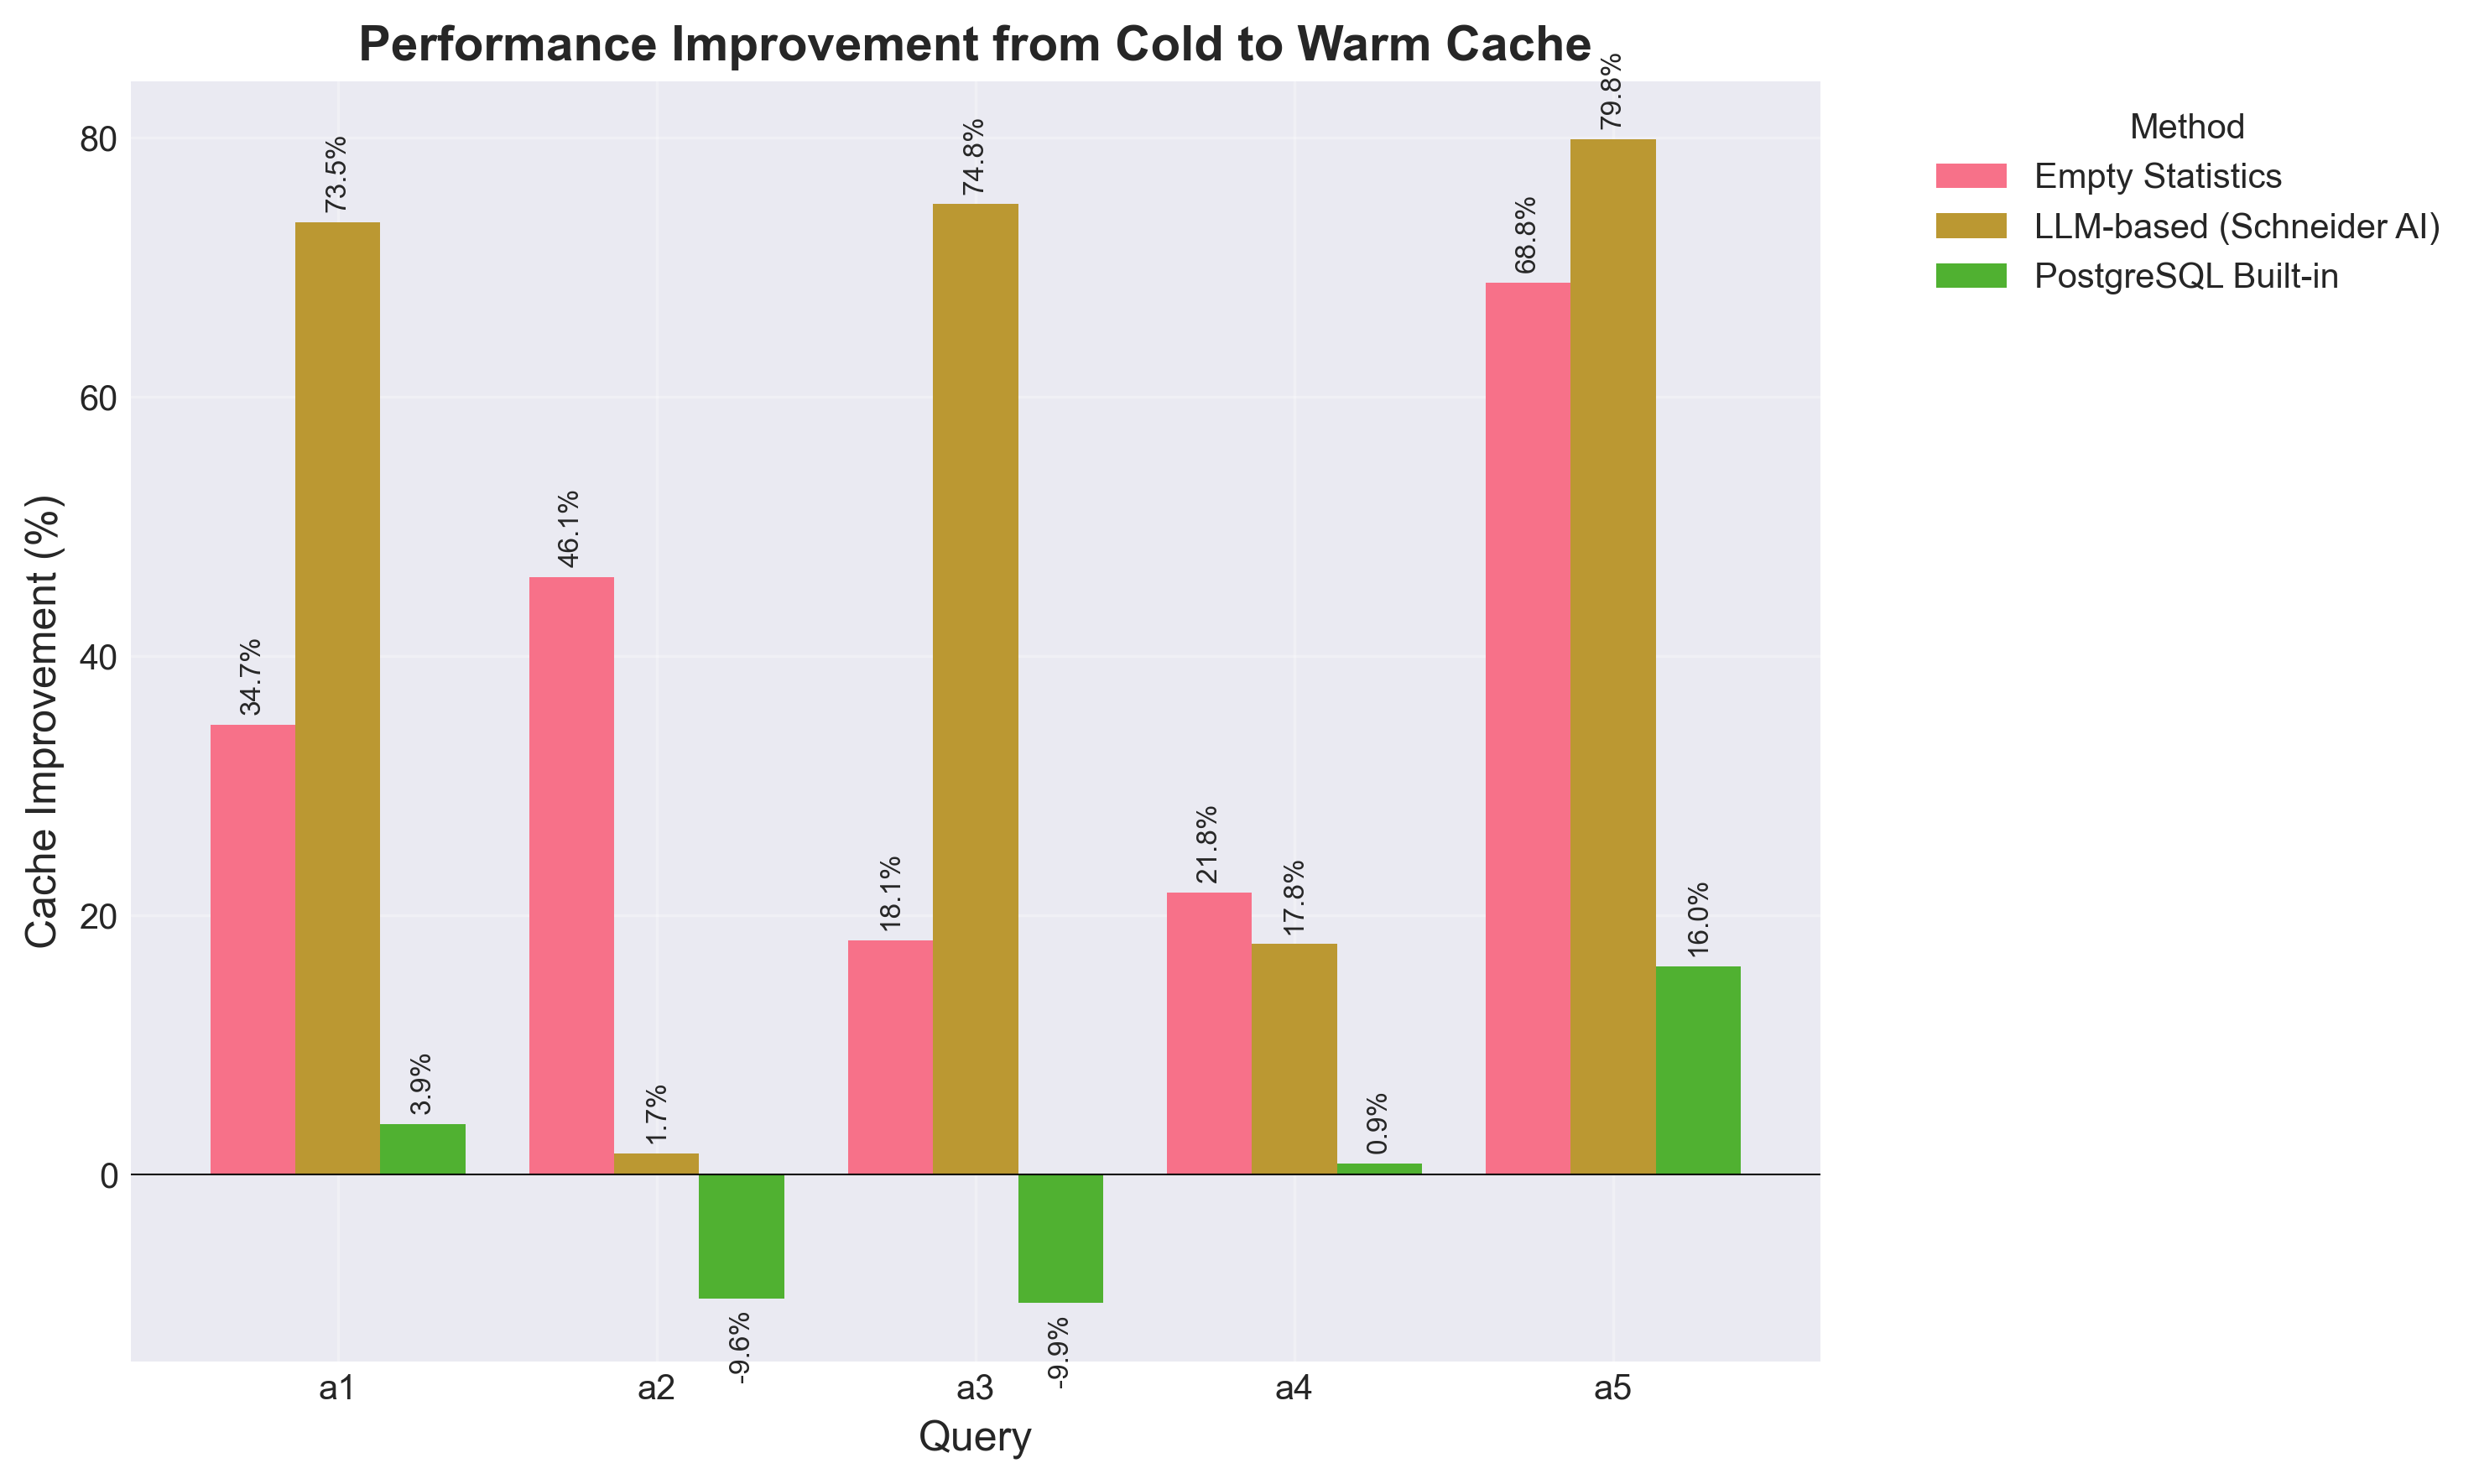
\includegraphics[width=0.9\textwidth]{images/cache_improvement_comparison.png}
\end{center}

\begin{exampleblock}{Cache Improvement Findings}
\begin{itemize}
    \item Percentage improvement from first trial to subsequent trials
    \item Negative values indicate performance degradation
    \item Variable cache effects suggest buffer management challenges
    \item Some queries show minimal cache benefit
\end{itemize}
\end{exampleblock}

\end{frame}

% Section 7: Discussion
\section{Discussion}

\begin{frame}{Privacy Guarantees}
\frametitle{Achieving $\varepsilon$-Differential Privacy}

\begin{block}{Privacy Model}
\begin{itemize}
    \item LLM never accesses actual data
    \item Statistics based on schema and domain knowledge only
    \item No information leakage about specific records
    \item Satisfies differential privacy definition
\end{itemize}
\end{block}

\begin{theorem}[Privacy Guarantee]
For any two adjacent databases $D$ and $D'$ differing in one record, and any statistics output $S$:
$$\Pr[\text{LLM}(schema) = S | D] = \Pr[\text{LLM}(schema) = S | D']$$
\end{theorem}

\begin{alertblock}{Implications}
\begin{itemize}
    \item Statistics reveal nothing about individual records
    \item Adversary cannot infer presence/absence of specific data
    \item Privacy preserved even with full statistics access
\end{itemize}
\end{alertblock}

\end{frame}

\begin{frame}{Limitations and Trade-offs}
\frametitle{Current Approach Constraints}

\begin{columns}[T]
\begin{column}{0.5\textwidth}
\begin{block}{Limitations}
\begin{itemize}
    \item Requires domain knowledge
    \item May miss unusual patterns
    \item LLM API costs
    \item Initial setup complexity
\end{itemize}
\end{block}
\end{column}

\begin{column}{0.5\textwidth}
\begin{block}{Trade-offs}
\begin{itemize}
    \item Privacy vs accuracy
    \item Generality vs specificity
    \item Cost vs performance
    \item Automation vs control
\end{itemize}
\end{block}
\end{column}
\end{columns}

\vspace{0.5cm}

\begin{exampleblock}{When to Use This Approach}
\begin{itemize}
    \item High privacy requirements
    \item Well-understood domain (e.g., e-commerce, social media)
    \item Moderate performance requirements
    \item Multi-tenant or sensitive databases
\end{itemize}
\end{exampleblock}

\end{frame}

% Section 8: Conclusions
\section{Conclusions}

\begin{frame}{Summary of Contributions}
\frametitle{What We Actually Accomplished}

\begin{enumerate}
    \item \textbf{Novel Exploration}: First systematic study of LLMs for privacy-preserving database statistics generation
    
    \item \textbf{Practical Implementation}: Working system integrated with PostgreSQL for rigorous testing
    
    \item \textbf{Honest Empirical Evaluation}: Revealed significant instability and performance issues with LLM-generated statistics
    
    \item \textbf{Privacy Analysis}: Demonstrated theoretical privacy guarantees without data access
    
    \item \textbf{Open Source Benchmarking Platform}: Extensible framework for future privacy-preserving query optimization research
\end{enumerate}

\vspace{0.5cm}

\begin{alertblock}{Realistic Impact}
While the LLM approach shows promise, our data indicates it's not yet ready for production. The benchmarking platform will be valuable for evaluating future privacy-preserving methods like DPOpt.
\end{alertblock}

\end{frame}

\begin{frame}{Key Findings}
\frametitle{What Our Data Actually Shows}

\begin{alertblock}{\Large LLM Statistics Are Highly Unstable}
\Large
\begin{itemize}
    \item LLM-generated statistics show significant variation between runs
    \item Can cause enormous performance penalties (e.g., Query a2: 3.36s vs 0.024s)
    \item On average, perform equal to or \textbf{worse} than simply erasing statistics
\end{itemize}
\end{alertblock}

\vspace{0.5cm}

\begin{block}{Reality Check}
\begin{itemize}
    \item Current LLM approach is not ready for production use
    \item Empty statistics baseline often more predictable
    \item Privacy comes at significant performance cost
    \item More research needed to make this approach viable
\end{itemize}
\end{block}

\end{frame}

\begin{frame}{Future Research Directions}
\frametitle{Next Steps for Privacy-Preserving Query Optimization}

\begin{block}{Improving LLM-Based Methods}
\begin{itemize}
    \item Fine-tuning models specifically for database statistics
    \item Developing consistency mechanisms across runs
    \item Better validation and error detection
\end{itemize}
\end{block}

\vspace{0.5cm}

\begin{alertblock}{Primary Future Direction: DPOpt Integration}
\Large
\textbf{DPOpt: Differentially Private Query Optimization}
\begin{itemize}
    \item Integrate test bench with Sara Alam's privacy-preserving database
    \item Secure implementations from SPECIAL: Synopsis Assisted Secure Collaborative Analytics
    \item More principled approach to differential privacy in query optimization
\end{itemize}
\end{alertblock}

\end{frame}

% Thank you slide
\begin{frame}
\begin{center}
\Huge Thank You!

\vspace{1cm}

\Large Questions?

\vspace{1cm}

\normalsize
\texttt{seth.lupo@tufts.edu}\\
\vspace{0.5cm}
Tufts Security and Privacy Lab

\end{center}
\end{frame}

\end{document}
